\documentclass{article}\usepackage[]{graphicx}\usepackage[]{color}
%% maxwidth is the original width if it is less than linewidth
%% otherwise use linewidth (to make sure the graphics do not exceed the margin)
\makeatletter
\def\maxwidth{ %
  \ifdim\Gin@nat@width>\linewidth
    \linewidth
  \else
    \Gin@nat@width
  \fi
}
\makeatother

\definecolor{fgcolor}{rgb}{0.345, 0.345, 0.345}
\newcommand{\hlnum}[1]{\textcolor[rgb]{0.686,0.059,0.569}{#1}}%
\newcommand{\hlstr}[1]{\textcolor[rgb]{0.192,0.494,0.8}{#1}}%
\newcommand{\hlcom}[1]{\textcolor[rgb]{0.678,0.584,0.686}{\textit{#1}}}%
\newcommand{\hlopt}[1]{\textcolor[rgb]{0,0,0}{#1}}%
\newcommand{\hlstd}[1]{\textcolor[rgb]{0.345,0.345,0.345}{#1}}%
\newcommand{\hlkwa}[1]{\textcolor[rgb]{0.161,0.373,0.58}{\textbf{#1}}}%
\newcommand{\hlkwb}[1]{\textcolor[rgb]{0.69,0.353,0.396}{#1}}%
\newcommand{\hlkwc}[1]{\textcolor[rgb]{0.333,0.667,0.333}{#1}}%
\newcommand{\hlkwd}[1]{\textcolor[rgb]{0.737,0.353,0.396}{\textbf{#1}}}%

\usepackage{framed}
\makeatletter
\newenvironment{kframe}{%
 \def\at@end@of@kframe{}%
 \ifinner\ifhmode%
  \def\at@end@of@kframe{\end{minipage}}%
  \begin{minipage}{\columnwidth}%
 \fi\fi%
 \def\FrameCommand##1{\hskip\@totalleftmargin \hskip-\fboxsep
 \colorbox{shadecolor}{##1}\hskip-\fboxsep
     % There is no \\@totalrightmargin, so:
     \hskip-\linewidth \hskip-\@totalleftmargin \hskip\columnwidth}%
 \MakeFramed {\advance\hsize-\width
   \@totalleftmargin\z@ \linewidth\hsize
   \@setminipage}}%
 {\par\unskip\endMakeFramed%
 \at@end@of@kframe}
\makeatother

\definecolor{shadecolor}{rgb}{.97, .97, .97}
\definecolor{messagecolor}{rgb}{0, 0, 0}
\definecolor{warningcolor}{rgb}{1, 0, 1}
\definecolor{errorcolor}{rgb}{1, 0, 0}
\newenvironment{knitrout}{}{} % an empty environment to be redefined in TeX

\usepackage{alltt}
\usepackage{float} 
\usepackage{booktabs}
\usepackage{longtable}
\usepackage{tabularx}
\usepackage{xcolor,colortbl}

\colorlet{tableheadcolor}{gray!50}
\newcommand{\headcol}{\rowcolor{tableheadcolor}}
\colorlet{tablerowcolor}{gray!25}
\newcommand{\rowcol}{\rowcolor{tablerowcolor}}

\usepackage{geometry}
\geometry{verbose, tmargin=2cm, bmargin=2cm, lmargin=2cm, rmargin=2cm}
\IfFileExists{upquote.sty}{\usepackage{upquote}}{}
\begin{document}



\title{Projected fire change 2000 - 2099 \\ \large Unvetted preliminary rush draft from developmental code}
\author{Matthew Leonawicz}
\maketitle

\setlength{\aboverulesep}{0.2pt}
\setlength{\belowrulesep}{0.2pt}



\section{Projected fire change tables}
In each subsection below, the third table down with percentages relates to table 8.1 in the original document.
This uses strictly ALFRESCO output.
The tables use years 2000 - 2009 and 2090 - 2099.
There is one section for each region, Alaska and the five LCCs.


\subsection{Alaska}
\subsubsection{Historical fire}

% latex table generated in R 3.1.1 by xtable 1.7-4 package
% Tue Jan 06 10:46:55 2015
\begin{table}[ht]
\centering
\begin{tabular}{lccc}
  \headcol 
 \toprule
Climate-change scenario & Percentile & Ignitions & Area burned \\ 
  \midrule
SRES B1 & 50th & 60 & 3398 \\ 
  SRES B1 & 95th & 86 & 18131 \\ 
  SRES A1B & 50th & 59 & 3066 \\ 
  SRES A1B & 95th & 85 & 17486 \\ 
  SRES A2 & 50th & 60 & 3242 \\ 
  SRES A2 & 95th & 84 & 17962 \\ 
   \bottomrule
\end{tabular}
\end{table}


\subsubsection{Projected fire}

% latex table generated in R 3.1.1 by xtable 1.7-4 package
% Tue Jan 06 10:46:55 2015
\begin{table}[ht]
\centering
\begin{tabular}{lccc}
  \headcol 
 \toprule
Climate-change scenario & Percentile & Ignitions & Area burned \\ 
  \midrule
SRES B1 & 50th & 60 & 2929 \\ 
  SRES B1 & 95th & 83 & 19079 \\ 
  SRES A1B & 50th & 62 & 5441 \\ 
  SRES A1B & 95th & 88 & 33039 \\ 
  SRES A2 & 50th & 66 & 3465 \\ 
  SRES A2 & 95th & 89 & 15350 \\ 
   \bottomrule
\end{tabular}
\end{table}


\subsubsection{Percent change}

% latex table generated in R 3.1.1 by xtable 1.7-4 package
% Tue Jan 06 10:46:55 2015
\begin{table}[ht]
\centering
\begin{tabular}{lccc}
  \headcol 
 \toprule
Climate-change scenario & Percentile & Ignitions & Area burned \\ 
  \midrule
SRES B1 & 50th & 0.8 & -13.8 \\ 
  SRES B1 & 95th & -2.6 & 5.2 \\ 
  SRES A1B & 50th & 4.2 & 77.5 \\ 
  SRES A1B & 95th & 4.4 & 89.0 \\ 
  SRES A2 & 50th & 9.2 & 6.9 \\ 
  SRES A2 & 95th & 5.2 & -14.5 \\ 
   \bottomrule
\end{tabular}
\end{table}


\newpage
\subsection{Arctic}
\subsubsection{Historical fire}

% latex table generated in R 3.1.1 by xtable 1.7-4 package
% Tue Jan 06 10:46:55 2015
\begin{table}[ht]
\centering
\begin{tabular}{lccc}
  \headcol 
 \toprule
Climate-change scenario & Percentile & Ignitions & Area burned \\ 
  \midrule
SRES B1 & 50th & 1 & 22 \\ 
  SRES B1 & 95th & 3 & 5935 \\ 
  SRES A1B & 50th & 1 & 10 \\ 
  SRES A1B & 95th & 4 & 5471 \\ 
  SRES A2 & 50th & 1 & 10 \\ 
  SRES A2 & 95th & 3 & 6347 \\ 
   \bottomrule
\end{tabular}
\end{table}


\subsubsection{Projected fire}

% latex table generated in R 3.1.1 by xtable 1.7-4 package
% Tue Jan 06 10:46:55 2015
\begin{table}[ht]
\centering
\begin{tabular}{lccc}
  \headcol 
 \toprule
Climate-change scenario & Percentile & Ignitions & Area burned \\ 
  \midrule
SRES B1 & 50th & 1 & 24 \\ 
  SRES B1 & 95th & 4 & 4207 \\ 
  SRES A1B & 50th & 1 & 134 \\ 
  SRES A1B & 95th & 4 & 8263 \\ 
  SRES A2 & 50th & 1 & 12 \\ 
  SRES A2 & 95th & 4 & 3068 \\ 
   \bottomrule
\end{tabular}
\end{table}


\subsubsection{Percent change}

% latex table generated in R 3.1.1 by xtable 1.7-4 package
% Tue Jan 06 10:46:55 2015
\begin{table}[ht]
\centering
\begin{tabular}{lccc}
  \headcol 
 \toprule
Climate-change scenario & Percentile & Ignitions & Area burned \\ 
  \midrule
SRES B1 & 50th & 0.0 & 9.1 \\ 
  SRES B1 & 95th & 18.3 & -29.1 \\ 
  SRES A1B & 50th & 0.0 & 1240.0 \\ 
  SRES A1B & 95th & 0.0 & 51.0 \\ 
  SRES A2 & 50th & 0.0 & 20.0 \\ 
  SRES A2 & 95th & 18.3 & -51.7 \\ 
   \bottomrule
\end{tabular}
\end{table}


\newpage
\subsection{North Pacific}
\subsubsection{Historical fire}

% latex table generated in R 3.1.1 by xtable 1.7-4 package
% Tue Jan 06 10:46:55 2015
\begin{table}[ht]
\centering
\begin{tabular}{lccc}
  \headcol 
 \toprule
Climate-change scenario & Percentile & Ignitions & Area burned \\ 
  \midrule
SRES B1 & 50th & 0 & 2 \\ 
  SRES B1 & 95th & 2 & 26 \\ 
  SRES A1B & 50th & 0 & 2 \\ 
  SRES A1B & 95th & 2 & 25 \\ 
  SRES A2 & 50th & 0 & 2 \\ 
  SRES A2 & 95th & 2 & 19 \\ 
   \bottomrule
\end{tabular}
\end{table}


\subsubsection{Projected fire}

% latex table generated in R 3.1.1 by xtable 1.7-4 package
% Tue Jan 06 10:46:55 2015
\begin{table}[ht]
\centering
\begin{tabular}{lccc}
  \headcol 
 \toprule
Climate-change scenario & Percentile & Ignitions & Area burned \\ 
  \midrule
SRES B1 & 50th & 0 & 2 \\ 
  SRES B1 & 95th & 2 & 22 \\ 
  SRES A1B & 50th & 0 & 5 \\ 
  SRES A1B & 95th & 3 & 186 \\ 
  SRES A2 & 50th & 0 & 4 \\ 
  SRES A2 & 95th & 2 & 44 \\ 
   \bottomrule
\end{tabular}
\end{table}


\subsubsection{Percent change}

% latex table generated in R 3.1.1 by xtable 1.7-4 package
% Tue Jan 06 10:46:55 2015
\begin{table}[ht]
\centering
\begin{tabular}{lccc}
  \headcol 
 \toprule
Climate-change scenario & Percentile & Ignitions & Area burned \\ 
  \midrule
SRES B1 & 50th & - & - \\ 
  SRES B1 & 95th & -22.5 & -15.38 \\ 
  SRES A1B & 50th & - & - \\ 
  SRES A1B & 95th & 64.52 & 644 \\ 
  SRES A2 & 50th & - & - \\ 
  SRES A2 & 95th & 0 & 131.58 \\ 
   \bottomrule
\end{tabular}
\end{table}


\newpage
\subsection{Northwest Interior Forest North}
\subsubsection{Historical fire}

% latex table generated in R 3.1.1 by xtable 1.7-4 package
% Tue Jan 06 10:46:55 2015
\begin{table}[ht]
\centering
\begin{tabular}{lccc}
  \headcol 
 \toprule
Climate-change scenario & Percentile & Ignitions & Area burned \\ 
  \midrule
SRES B1 & 50th & 42 & 2255 \\ 
  SRES B1 & 95th & 62 & 10642 \\ 
  SRES A1B & 50th & 42 & 2203 \\ 
  SRES A1B & 95th & 62 & 10536 \\ 
  SRES A2 & 50th & 42 & 2270 \\ 
  SRES A2 & 95th & 61 & 10507 \\ 
   \bottomrule
\end{tabular}
\end{table}


\subsubsection{Projected fire}

% latex table generated in R 3.1.1 by xtable 1.7-4 package
% Tue Jan 06 10:46:55 2015
\begin{table}[ht]
\centering
\begin{tabular}{lccc}
  \headcol 
 \toprule
Climate-change scenario & Percentile & Ignitions & Area burned \\ 
  \midrule
SRES B1 & 50th & 46 & 2223 \\ 
  SRES B1 & 95th & 65 & 10164 \\ 
  SRES A1B & 50th & 45 & 3292 \\ 
  SRES A1B & 95th & 65 & 16612 \\ 
  SRES A2 & 50th & 47 & 2527 \\ 
  SRES A2 & 95th & 66 & 8025 \\ 
   \bottomrule
\end{tabular}
\end{table}


\subsubsection{Percent change}

% latex table generated in R 3.1.1 by xtable 1.7-4 package
% Tue Jan 06 10:46:55 2015
\begin{table}[ht]
\centering
\begin{tabular}{lccc}
  \headcol 
 \toprule
Climate-change scenario & Percentile & Ignitions & Area burned \\ 
  \midrule
SRES B1 & 50th & 7.1 & -1.4 \\ 
  SRES B1 & 95th & 4.4 & -4.5 \\ 
  SRES A1B & 50th & 8.4 & 49.4 \\ 
  SRES A1B & 95th & 4.4 & 57.7 \\ 
  SRES A2 & 50th & 10.6 & 11.3 \\ 
  SRES A2 & 95th & 7.3 & -23.6 \\ 
   \bottomrule
\end{tabular}
\end{table}


\newpage
\subsection{Northwest Interior Forest South}
\subsubsection{Historical fire}

% latex table generated in R 3.1.1 by xtable 1.7-4 package
% Tue Jan 06 10:46:55 2015
\begin{table}[ht]
\centering
\begin{tabular}{lccc}
  \headcol 
 \toprule
Climate-change scenario & Percentile & Ignitions & Area burned \\ 
  \midrule
SRES B1 & 50th & 10 & 268 \\ 
  SRES B1 & 95th & 20 & 2240 \\ 
  SRES A1B & 50th & 10 & 204 \\ 
  SRES A1B & 95th & 20 & 2308 \\ 
  SRES A2 & 50th & 10 & 198 \\ 
  SRES A2 & 95th & 20 & 2346 \\ 
   \bottomrule
\end{tabular}
\end{table}


\subsubsection{Projected fire}

% latex table generated in R 3.1.1 by xtable 1.7-4 package
% Tue Jan 06 10:46:55 2015
\begin{table}[ht]
\centering
\begin{tabular}{lccc}
  \headcol 
 \toprule
Climate-change scenario & Percentile & Ignitions & Area burned \\ 
  \midrule
SRES B1 & 50th & 9 & 164 \\ 
  SRES B1 & 95th & 18 & 1364 \\ 
  SRES A1B & 50th & 10 & 411 \\ 
  SRES A1B & 95th & 22 & 12503 \\ 
  SRES A2 & 50th & 11 & 268 \\ 
  SRES A2 & 95th & 20 & 2139 \\ 
   \bottomrule
\end{tabular}
\end{table}


\subsubsection{Percent change}

% latex table generated in R 3.1.1 by xtable 1.7-4 package
% Tue Jan 06 10:46:55 2015
\begin{table}[ht]
\centering
\begin{tabular}{lccc}
  \headcol 
 \toprule
Climate-change scenario & Percentile & Ignitions & Area burned \\ 
  \midrule
SRES B1 & 50th & -14.3 & -38.8 \\ 
  SRES B1 & 95th & -10.2 & -39.1 \\ 
  SRES A1B & 50th & 10.5 & 101.5 \\ 
  SRES A1B & 95th & 10.2 & 441.7 \\ 
  SRES A2 & 50th & 15.8 & 35.4 \\ 
  SRES A2 & 95th & -1.0 & -8.8 \\ 
   \bottomrule
\end{tabular}
\end{table}


\newpage
\subsection{Western Alaska}
\subsubsection{Historical fire}

% latex table generated in R 3.1.1 by xtable 1.7-4 package
% Tue Jan 06 10:46:55 2015
\begin{table}[ht]
\centering
\begin{tabular}{lccc}
  \headcol 
 \toprule
Climate-change scenario & Percentile & Ignitions & Area burned \\ 
  \midrule
SRES B1 & 50th & 9 & 736 \\ 
  SRES B1 & 95th & 17 & 7672 \\ 
  SRES A1B & 50th & 8 & 316 \\ 
  SRES A1B & 95th & 17 & 6787 \\ 
  SRES A2 & 50th & 8 & 364 \\ 
  SRES A2 & 95th & 17 & 8077 \\ 
   \bottomrule
\end{tabular}
\end{table}


\subsubsection{Projected fire}

% latex table generated in R 3.1.1 by xtable 1.7-4 package
% Tue Jan 06 10:46:55 2015
\begin{table}[ht]
\centering
\begin{tabular}{lccc}
  \headcol 
 \toprule
Climate-change scenario & Percentile & Ignitions & Area burned \\ 
  \midrule
SRES B1 & 50th & 7 & 364 \\ 
  SRES B1 & 95th & 16 & 9236 \\ 
  SRES A1B & 50th & 8 & 936 \\ 
  SRES A1B & 95th & 16 & 10232 \\ 
  SRES A2 & 50th & 8 & 936 \\ 
  SRES A2 & 95th & 17 & 8516 \\ 
   \bottomrule
\end{tabular}
\end{table}


\subsubsection{Percent change}

% latex table generated in R 3.1.1 by xtable 1.7-4 package
% Tue Jan 06 10:46:55 2015
\begin{table}[ht]
\centering
\begin{tabular}{lccc}
  \headcol 
 \toprule
Climate-change scenario & Percentile & Ignitions & Area burned \\ 
  \midrule
SRES B1 & 50th & -22.2 & -50.5 \\ 
  SRES B1 & 95th & -7.9 & 20.4 \\ 
  SRES A1B & 50th & -5.9 & 196.2 \\ 
  SRES A1B & 95th & -5.9 & 50.8 \\ 
  SRES A2 & 50th & 6.2 & 157.1 \\ 
  SRES A2 & 95th & 0.0 & 5.4 \\ 
   \bottomrule
\end{tabular}
\end{table}


\newpage
\section{Percentile fire trends by scenario}
The below graph relates to figure 8.2 in the original document.
This uses strictly ALFRESCO output.
\subsection{Alaska}
\begin{figure}[H]
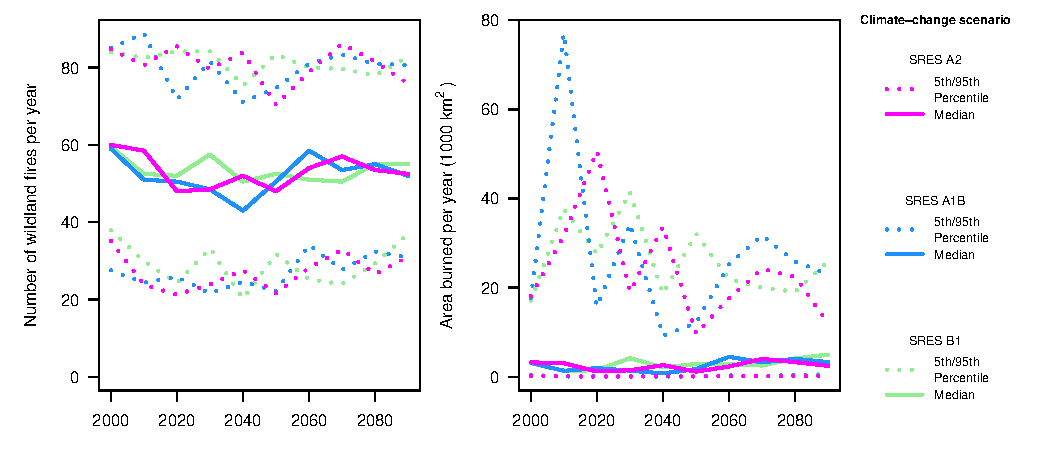
\includegraphics[width=\maxwidth]{figure/fire_change_ts_AK-1} \caption[Alaska]{Alaska\label{fig:fire_change_ts_AK}}
\end{figure}



All five following separate LCC graphs relate to figure 8.3 in the original document.
This uses strictly ALFRESCO output.
\subsection{Arctic}
\begin{figure}[H]
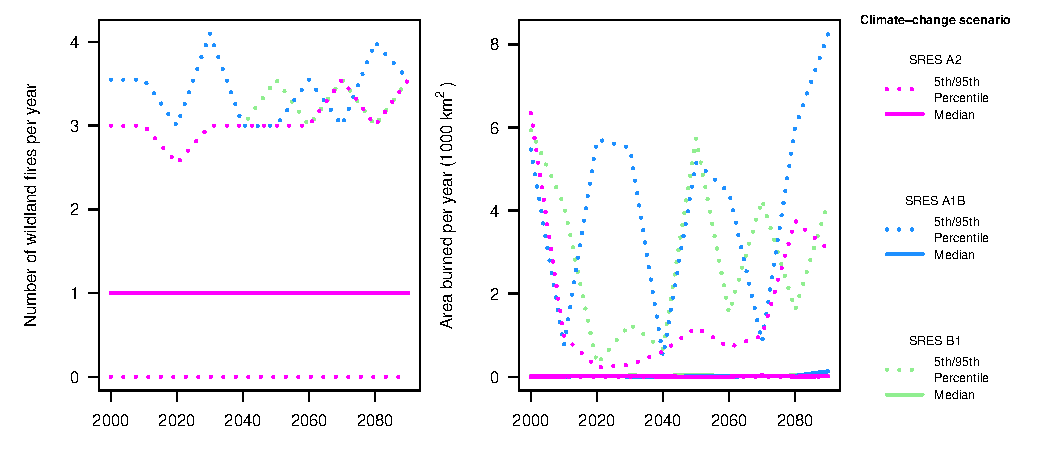
\includegraphics[width=\maxwidth]{figure/fire_change_ts_LCC1-1} \caption[Arctic]{Arctic\label{fig:fire_change_ts_LCC1}}
\end{figure}



\subsection{North Pacific}
\begin{figure}[H]
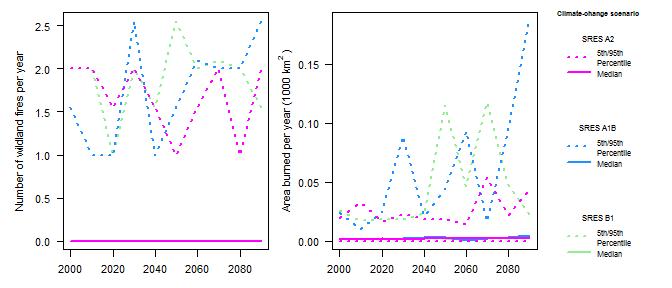
\includegraphics[width=\maxwidth]{figure/fire_change_ts_LCC2-1} \caption[North Pacific]{North Pacific\label{fig:fire_change_ts_LCC2}}
\end{figure}



\subsection{Northwest Interior Forest North}
\begin{figure}[H]
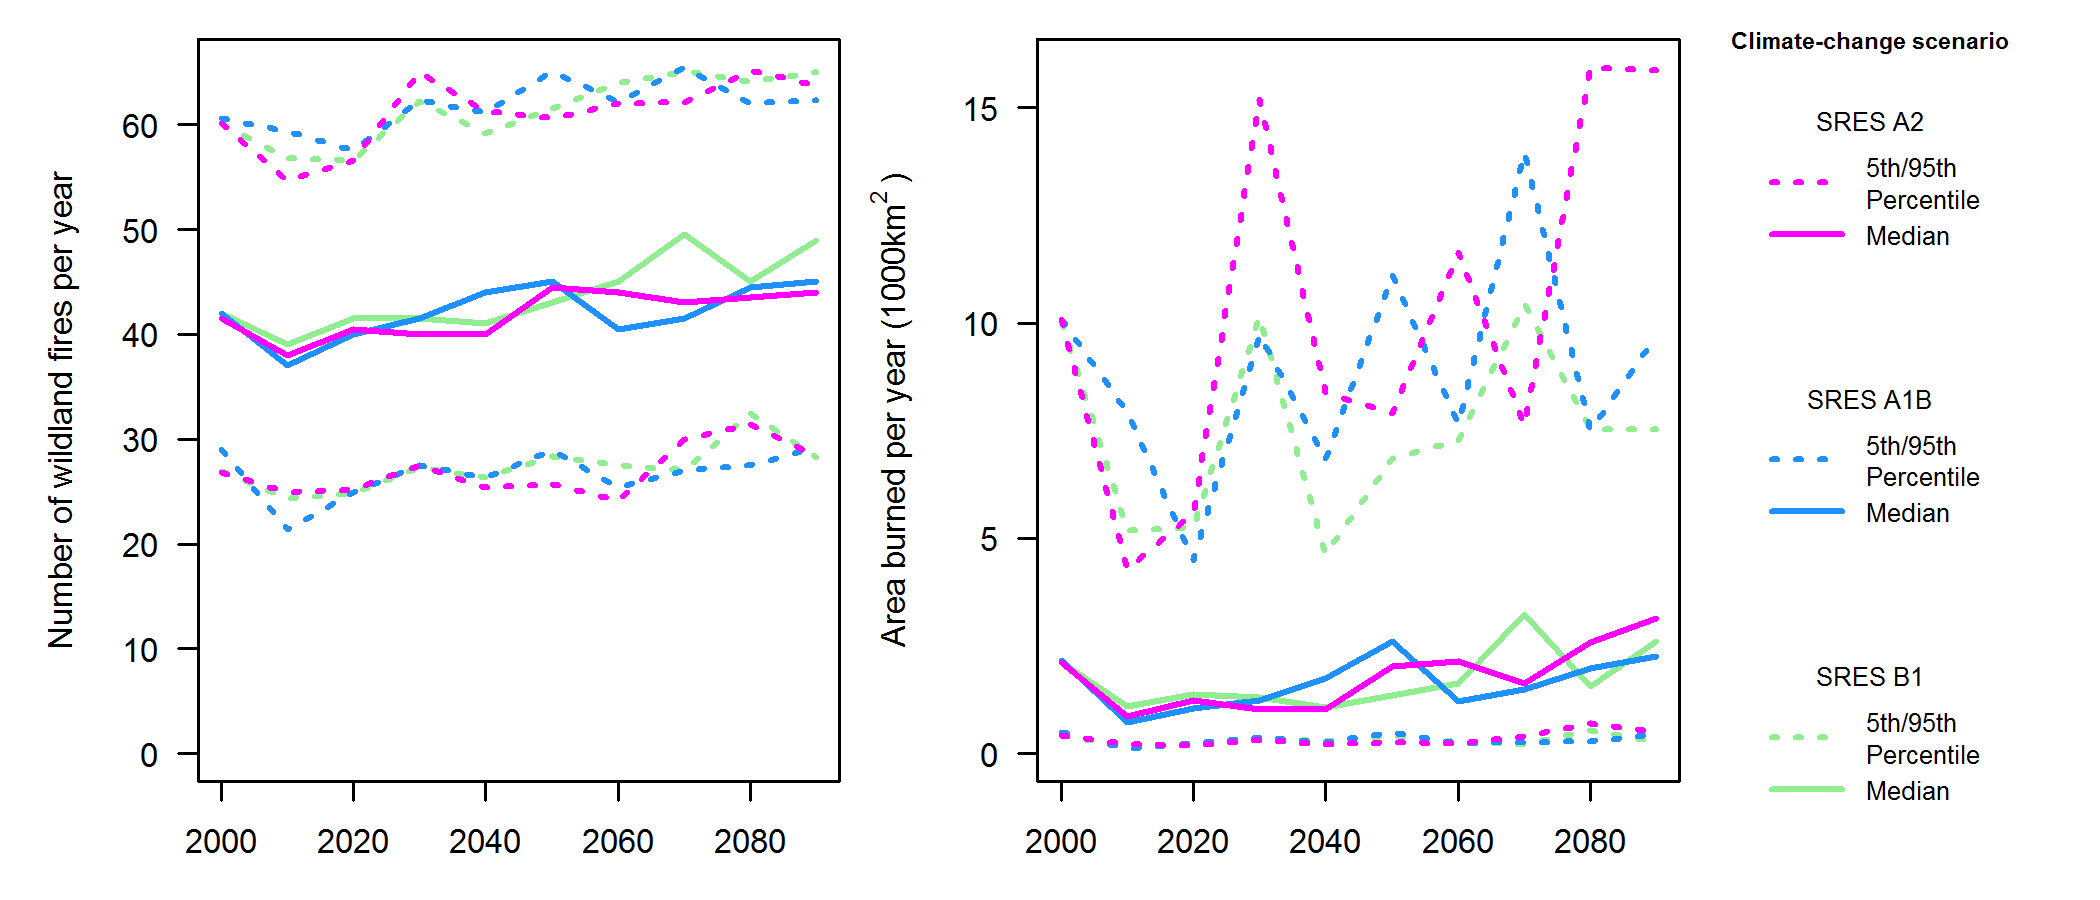
\includegraphics[width=\maxwidth]{figure/fire_change_ts_LCC3-1} \caption[Northwest Interior Forest North]{Northwest Interior Forest North\label{fig:fire_change_ts_LCC3}}
\end{figure}



\subsection{Northwest Interior Forest South}
\begin{figure}[H]
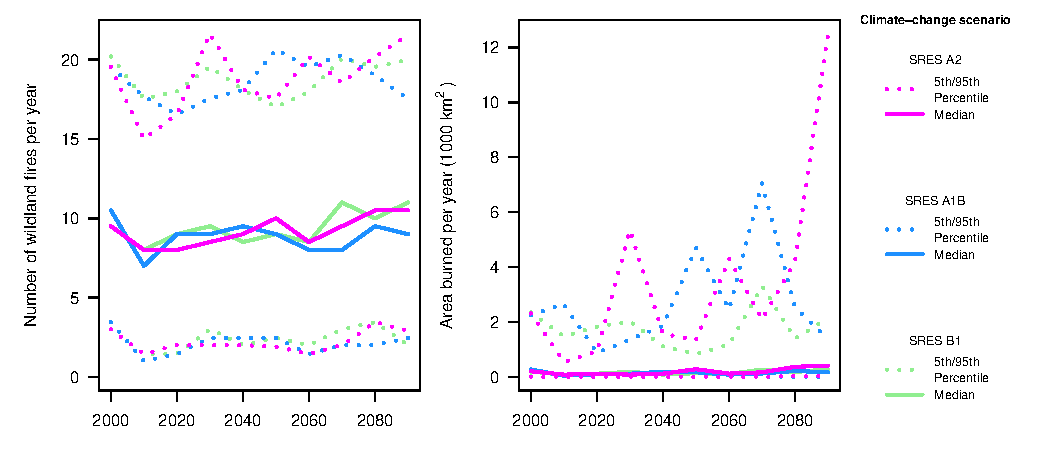
\includegraphics[width=\maxwidth]{figure/fire_change_ts_LCC4-1} \caption[Northwest Interior Forest South]{Northwest Interior Forest South\label{fig:fire_change_ts_LCC4}}
\end{figure}



\subsection{Western Alaska}
\begin{figure}[H]
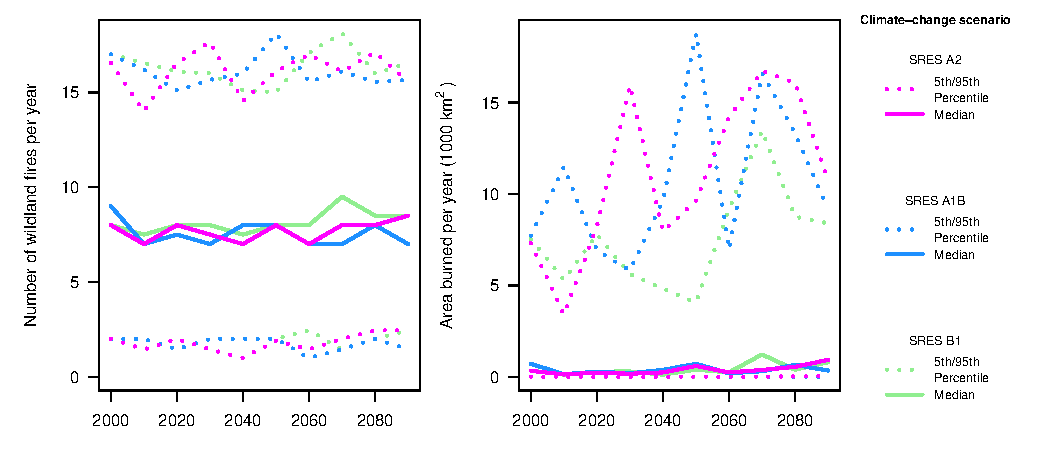
\includegraphics[width=\maxwidth]{figure/fire_change_ts_LCC5-1} \caption[Western Alaska]{Western Alaska\label{fig:fire_change_ts_LCC5}}
\end{figure}



\end{document}
